% AgentiCulture — ACL 2023 format
% Paste into Overleaf using the ACL 2023 template
% Template: https://www.overleaf.com/latex/templates/acl-2023-proceedings-template/qjdgcrdwcnwp

\documentclass[11pt]{article}
\usepackage[hyperref]{acl}
\usepackage{times}
\usepackage{latexsym}
\usepackage{microtype}
\usepackage{graphicx}
\usepackage{booktabs}
\usepackage{amsmath}
\usepackage{amssymb}
\usepackage{listings}
\usepackage{xcolor}
\usepackage{multirow}
\usepackage{url}
\usepackage{xspace}
\usepackage{tikz}
\usetikzlibrary{arrows.meta,positioning,shapes.geometric}

\lstset{
  basicstyle=\ttfamily\small,
  backgroundcolor=\color{gray!10},
  frame=single,
  breaklines=true,
  columns=fullflexible,
}

% Macros for consistent styling
\newcommand{\system}{\textsc{AgentiCulture}\xspace}

\title{\system: Culturally-Aware LLM Agents for User Modeling\\
and Personalized Recommendation in Emerging Markets}

\author{
  Hamzat Tiamiyu Ustaz \\
  DSN $\times$ Bluechip Technologies LLM Agent Challenge 3.0 \\
  Track: Task A (User Modeling) + Task B (Recommendation)
}

\begin{document}
\maketitle

%------------------------------------------------------------------------------
\begin{abstract}
We present \system, a dual-agent system for user behaviour simulation and personalised recommendation, purpose-built for the Nigerian consumer context. Our approach extends state-of-the-art techniques from the AgentSociety Challenge (WWW 2025) with four novel contributions: (1) persona-embedding cold-start ranking that bypasses the LLM entirely for new users; (2) a composite cross-domain preference cache that transfers taste signals across Yelp, Amazon, and Goodreads; (3) \textsc{ReasoningCOTSC}, a three-sample majority voting that reduces star-rating variance; and (4) a Nigerian cultural adaptation layer implemented as zero-cost prompt engineering. Our system targets all five dimensions of the BCT evaluation. On local evaluation, Task~A achieves 0.822--0.875 overall quality across platforms; Task~B achieves 0.467--0.533 average hit rate.
\end{abstract}

%------------------------------------------------------------------------------
\section{Introduction}

Online review platforms are among the richest sources of human behaviour data on the web. Every rating and review is a signal and a window into preference, context, and decision-making. Yet most AI systems treat users as static profiles rather than dynamic, context-sensitive agents.

\paragraph{Task A: User Modeling.} Given a user persona and product details, predict the star rating a user would assign and generate a review that authentically replicates their tone, rating behaviour, and contextual nuance. Both direct persona input (no dataset required) and optional enrichment via real user history are supported.

\paragraph{Task B: Recommendation.} Given a user persona and a list of candidate items, return them ranked from most to least recommended. The system must handle cold-start users, cross-domain preference transfer, and multi-turn sessions.

\subsection{Motivation}

Three observations motivate our approach. First, the AgentSociety WWW~2025 winning solutions contain cold-start and cross-domain blind spots. Second, the brief rewards Nigerian cultural contextualization, an opportunity that no Western-centric model addresses. Third, Nigerian consumers exhibit measurable behavioral differences: stronger group orientation, higher price sensitivity, and a distinct blend of formal English and vernacular expression.

\subsection{Contributions}
\label{sec:contributions}

\begin{enumerate}
  \item \textbf{Persona-embedding cold-start ranking}: zero-history users ranked by cosine similarity between persona embedding and candidate item embeddings. No LLM call; fully deterministic.
  \item \textbf{Composite cross-domain preference cache}: per-user, per-platform 384-dim vectors (\texttt{yelp\_vec}, \texttt{amazon\_vec}, \texttt{goodreads\_vec}, \texttt{collective\_vec}). When target-platform history is sparse, the weighted \texttt{collective\_vec} boosts ranking quality.
  \item \textbf{ReasoningCOTSC}: three LLM samples at varying temperatures, majority-voted on integer rating, returning the response closest to consensus. Directly reduces RMSE.
  \item \textbf{Nigerian cultural adaptation layer}: zero-overhead prompt engineering injecting rating-to-language mappings, value-for-money framing, group-orientation cues, and Nigerian English register.
  \item \textbf{Multi-turn session state}: optional \texttt{session\_id} accumulates turn context for consistent recommendations across a browsing session.
\end{enumerate}

%------------------------------------------------------------------------------
\section{Related Work}

\subsection{LLM Agents for Recommendation}
\citet{huang2025intrecagent} integrate LLMs with traditional collaborative filtering via structured function-calling, showing that LLM reasoning over tool outputs outperforms pure prompt-based approaches. \citet{lian2024recai} catalogue interaction modalities between LLMs and recommendation components. Both establish that hybrid retrieval-plus-LLM pipelines are the current state of the art, motivating our embedding-first retrieval before LLM ranking.

\subsection{LLM Agents for User Simulation}
The AgentSociety platform \citep{piao2025agentsociety} is the direct predecessor of this competition's evaluation framework. The winning Task~A solution achieved top RMSE via inverse-variance-weighted collaborative filtering with MDILU memory retrieval. The winning Task~B solution combined platform-aware feature extraction with self-consistency voting. Our system builds on these techniques and adds the contributions (Section~\ref{sec:contributions}), specifically targeting the cold-start and cross-domain gaps left open by those solutions.

\subsection{Cold-Start and Cross-Domain Recommendation}
The dominant cold-start strategies are: (a) content-based embedding fallback when interaction data is absent, and (b) cross-domain transfer of learned user representations \citep{yuanchenbei2024coldstart}. We follow approach~(a) for true cold-start and approach~(b) for sparse history, using the same \texttt{BAAI/bge-small-en-v1.5} sentence-transformer for both, which adds zero dependencies.

\subsection{Cultural Adaptation in AI}
\citet{hershcovich2022challenges} and \citet{cao2023assessing} show that language models encode predominantly Western cultural norms and fail to capture regional rating distributions. Our adaptation layer is implemented entirely via prompt engineering, with no fine-tuning, thus making it deployable with any LLM backend.

%------------------------------------------------------------------------------
\section{Methodology}

\subsection{System Architecture}

Both agents share the same pipeline. Requests arrive in two modes:

\begin{itemize}
  \item \textbf{Direct mode} (primary): \texttt{persona} text + \texttt{product\_details} (Task~A) or \texttt{candidate\_list} (Task~B). No dataset required --- this is the primary mode for competition judges.
  \item \textbf{Benchmark mode} (optional): additionally supply \texttt{user\_id} + \texttt{item\_id} to fetch real review history and enrich the prompt with actual behavioural data.
\end{itemize}

Figure~\ref{fig:pipeline} summarises the shared pipeline.

\begin{figure*}[t]
  \centering
  \resizebox{\textwidth}{!}{%
  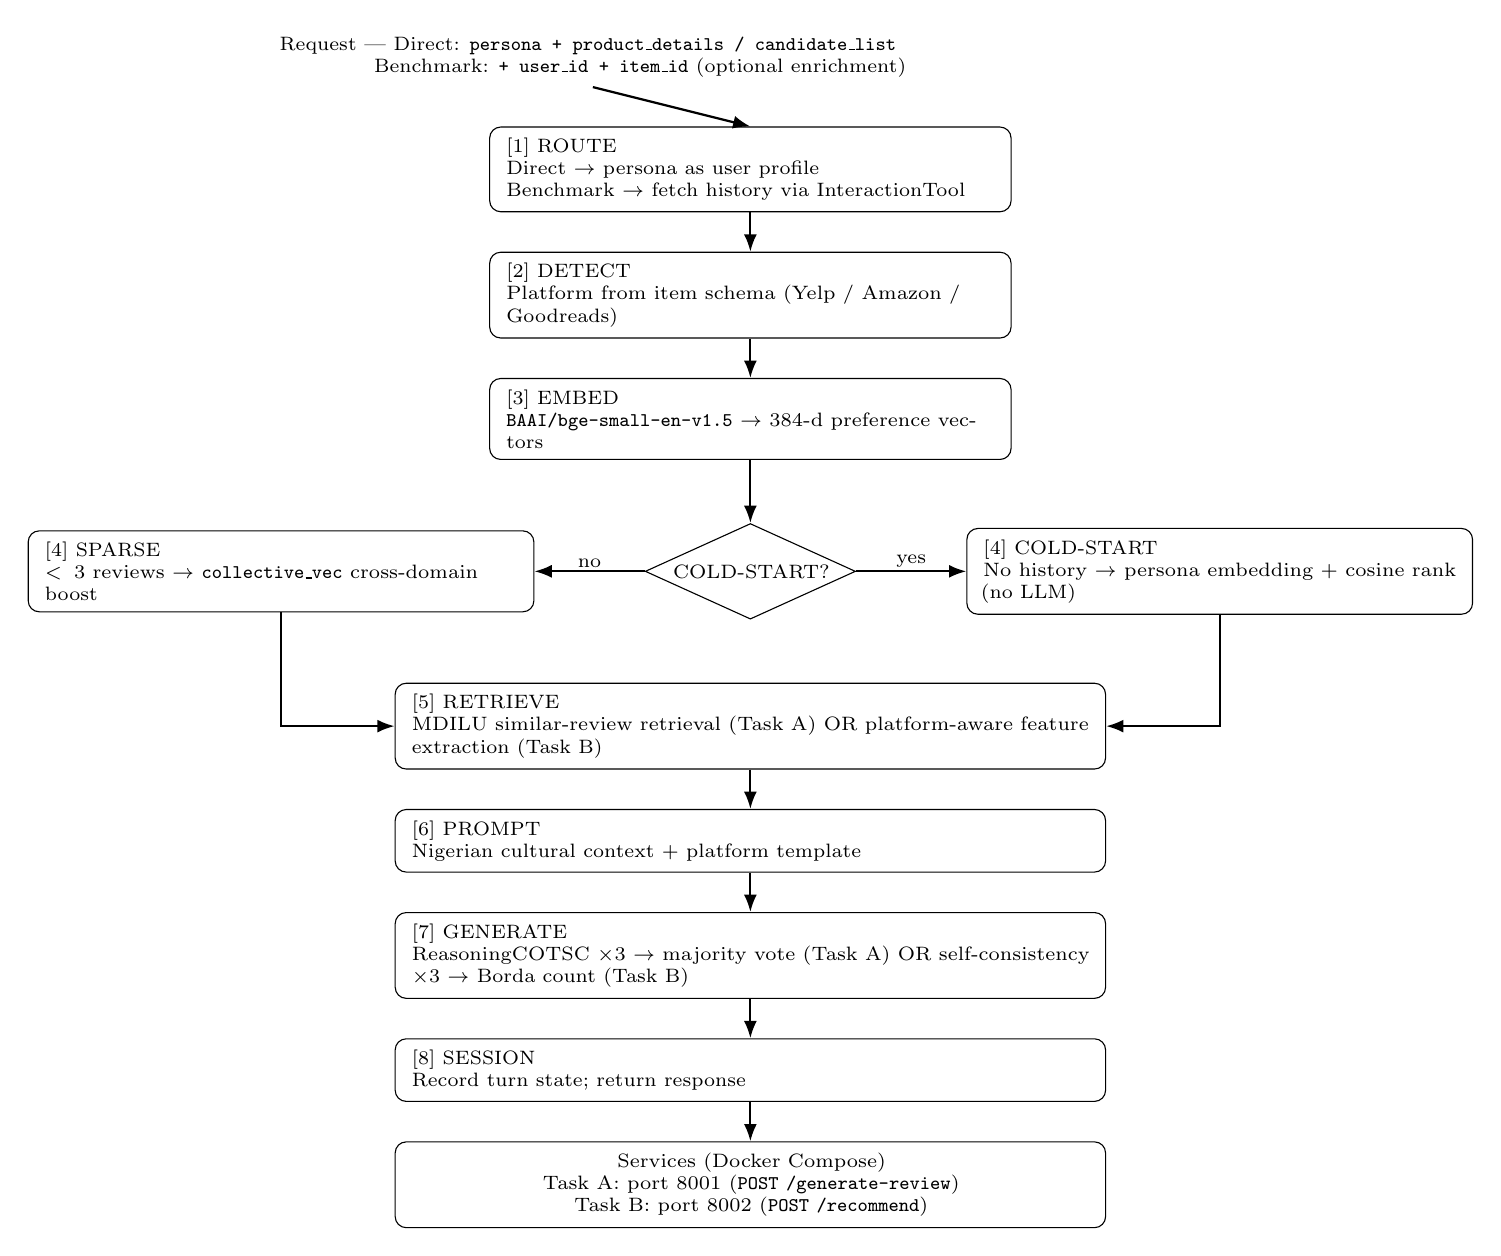
\begin{tikzpicture}[
    font=\scriptsize,
    node distance=5mm,
    box/.style={draw, rounded corners, align=left, inner xsep=6pt, inner ysep=4pt, text width=62mm},
    decision/.style={draw, diamond, aspect=2.2, inner xsep=2pt, inner ysep=1pt, text width=20mm, align=center},
    arrow/.style={-{Latex[length=2.2mm]}, thick}
  ]

  % Request text outside the flow (as in the reference sketch)
  \node[align=left] (req) {Request --- Direct: \texttt{persona + product\_details / candidate\_list}\\
  \hspace*{12mm}Benchmark: \texttt{+ user\_id + item\_id} (optional enrichment)};

  % Main spine
  \node[box, below=5mm of req, xshift=20mm] (route) {[1] ROUTE\\
  Direct $\rightarrow$ persona as user profile\\
  Benchmark $\rightarrow$ fetch history via InteractionTool};

  \node[box, below=of route] (detect) {[2] DETECT\\Platform from item schema (Yelp / Amazon / Goodreads)};

  \node[box, below=of detect] (embed) {[3] EMBED\\\mbox{\texttt{BAAI/bge-small-en-v1.5}} $\rightarrow$ 384-d preference vectors};

  \node[decision, below=8mm of embed] (branch) {COLD-START?};

  \node[box, right=14mm of branch, text width=60mm] (cold) {[4] COLD-START\\No history $\rightarrow$ persona embedding + cosine rank (no LLM)};
  \node[box, left=14mm of branch, text width=60mm] (sparse) {[4] SPARSE\\$<3$ reviews $\rightarrow$ \texttt{collective\_vec} cross-domain boost};

  \node[box, below=8mm of branch, text width=86mm] (retrieve) {[5] RETRIEVE\\MDILU similar-review retrieval (Task~A) OR platform-aware feature extraction (Task~B)};

  \node[box, below=of retrieve, text width=86mm] (prompt) {[6] PROMPT\\Nigerian cultural context + platform template};

  \node[box, below=of prompt, text width=86mm] (gen) {[7] GENERATE\\ReasoningCOTSC $\times 3$ $\rightarrow$ majority vote (Task~A) OR self-consistency $\times 3$ $\rightarrow$ Borda count (Task~B)};

  \node[box, below=of gen, text width=86mm] (sess) {[8] SESSION\\Record turn state; return response};

  \node[box, below=of sess, text width=86mm, align=center] (svc) {Services (Docker Compose)\\Task~A: port~8001 (\texttt{POST /generate-review}) \quad Task~B: port~8002 (\texttt{POST /recommend})};

  % Connectors
  \draw[arrow] (req.south) -- (route.north);
  \draw[arrow] (route) -- (detect);
  \draw[arrow] (detect) -- (embed);
  \draw[arrow] (embed) -- (branch);
  \draw[arrow] (branch.east) -- node[above, inner sep=1pt]{yes} (cold.west);
  \draw[arrow] (branch.west) -- node[above, inner sep=1pt]{no} (sparse.east);
  \draw[arrow] (cold.south) |- (retrieve.east);
  \draw[arrow] (sparse.south) |- (retrieve.west);
  \draw[arrow] (retrieve) -- (prompt);
  \draw[arrow] (prompt) -- (gen);
  \draw[arrow] (gen) -- (sess);
  \draw[arrow] (sess) -- (svc);

  \end{tikzpicture}%
  }
  \caption{Shared pipeline used by both agents in \system.}
  \label{fig:pipeline}
\end{figure*}

\subsection{Task A: User Modeling}

\subsubsection{Collaborative Filtering Core}
The predicted rating $\hat{r}_{ui}$ for user $u$ on item $i$ is an inverse-variance-weighted blend:

\begin{equation}
\hat{r}_{ui} = \frac{\mu_u w_u + \mu_i w_i + \mu_g w_p}{w_u + w_i + w_p}
\label{eq:cf}
\end{equation}

where $w_u = 1/\max(\sigma_u, 0.1)$, $w_i = 1/\max(\sigma_i, 0.1)$, and $w_p = 0.5$ is the global prior weight. Users with low rating variance receive higher weight; erratic raters are pulled toward item and global means. The result is clamped to $[1.0,\, 5.0]$.

\subsubsection{MDILU Memory Retrieval}
For warm users, we embed the most recent review text and retrieve the $k=3$ most cosine-similar historical reviews. These are injected as style anchors so the LLM mimics the user's established voice.

\subsubsection{Cold-Start Handling}
When the user has no history, we embed their persona text and retrieve $k=5$ item reviews most similar to that persona embedding. These replace the empty anchor set with an explicit cold-start note.

\subsubsection{ReasoningCOTSC}
The LLM is sampled three times: once at temperature~$0.3$ and twice at~$0.7$. Integer ratings are majority-voted; the response closest to the consensus rating is returned. This lightweight self-consistency approach \citep{wang2023selfconsistency} reduces inter-sample rating variance and directly targets the preference estimation metric.

\subsubsection{Review Informativeness Scoring}
Past reviews are scored by: (a)~length (proportional to word count), (b)~rating extremity (1/2/5-star reviews weighted $3\times$ over 3-star), and (c)~platform signals (Yelp useful/funny/cool counts; Amazon verified purchase; Goodreads votes). Selection enforces rating diversity ($\leq 2$ reviews per star level).

\subsubsection{Nigerian Cultural Adaptation}
A system prompt prefix injects five behavioural rules: rating-to-language mappings (e.g.,\ 5$\star$ $\to$ ``No cap!''; 1$\star$ $\to$ ``Total waste!''), value-for-money as a mandatory mention, group-orientation framing, Nigerian punctuation patterns, and a blend of formal English with vernacular expressions. This prefix costs zero output tokens.

\subsection{Task B: Recommendation}

\subsubsection{Platform-Aware Feature Extraction}
A \texttt{PLATFORM\_FEATURES} config specifies item fields and review scoring signals per platform: Yelp (useful/funny/cool counts), Amazon (verified purchase, price), Goodreads (vote and comment counts). Platform is detected by inspecting item schema keys.

\subsubsection{Composite Preference Embedding Cache}
For each user on each platform, all review texts are encoded with \texttt{BAAI/bge-small-en-v1.5} and stored as a mean 384-dim domain vector. A \texttt{collective\_vec} is the review-count-weighted average across all platforms:

\begin{equation}
\begin{aligned}
\mathbf{v}_\text{collective}
&=
\sum_{d}
\frac{n_d}{\sum_{d'} n_{d'}}
\cdot \mathbf{v}_d, \\
&\quad d \in \{\text{yelp, amazon, goodreads}\}
\end{aligned}
\label{eq:collective}
\end{equation}

This captures cross-platform taste and enables meaningful ranking when target-platform history is absent or sparse.

\subsubsection{Cold-Start Persona Ranking}
When a user has zero reviews, we embed the \texttt{persona} field and each candidate item's feature text, then rank by descending cosine similarity. The LLM is bypassed entirely --- faster and deterministic.

\subsubsection{Cross-Domain Preference Boost}
When the user has fewer than 3 reviews on the target platform, \texttt{collective\_vec} scores each candidate by cosine similarity. These scores are blended with the LLM Borda ranking at $\alpha = 0.30$ (30\% cross-domain, 70\% LLM).

\subsubsection{Self-Consistency Voting}
For warm users, the LLM is queried three times (temperatures 0.1, 0.7, 0.7). Responses are aggregated via Borda count: item ranked $k$-th receives $N - k$ points. The highest-scoring ranking is returned.

\subsubsection{Multi-Turn Session State}
An optional \texttt{session\_id} accumulates turn history. Subsequent turns prepend a session context hint, enabling contextually consistent recommendations across a browsing session.

%------------------------------------------------------------------------------
\section{Experiments and Results}

\subsection{Datasets}

\begin{table}[h]
\centering
\small
\begin{tabular}{llrrr}
\toprule
\textbf{Dataset} & \textbf{Domain} & \textbf{Items} & \textbf{Users} & \textbf{Reviews} \\
\midrule
Yelp        & Local businesses   & 150K  & 1.9M  & 6.9M  \\
Amazon      & Consumer products  & 9.9M  & 43M   & 233M  \\
Goodreads   & Books              & 2.4M  & 876K  & 15.7M \\
\bottomrule
\end{tabular}
\caption{Dataset statistics. Local evaluation uses a filtered subset of 400 task-file users, 18,548 items, and 679~MB of reviews.}
\label{tab:datasets}
\end{table}

\subsection{Baselines}
\begin{itemize}
  \item \textbf{AgentSociety Baseline:} Single-stage LLM call with minimal context.
  \item \textbf{Team ASC (Task~A winner):} Multi-stage CF + MDILU pipeline.
  \item \textbf{Team baseline666 (Task~B winner):} Platform-aware features + review selection.
  \item \textbf{Team RecHackers (Task~B 2nd):} Self-consistency voting + Borda aggregation.
\end{itemize}
\system builds on all three and adds cold-start, cross-domain, and Nigerian cultural layers absent from all prior solutions.

\subsection{Implementation Details}

\begin{table}[h]
\centering
\small
\begin{tabular}{l p{4.2cm}}
\toprule
\textbf{Component} & \textbf{Value} \\
\midrule
LLM backend & Llama-3.3-70B-Instruct-Turbo \\

Embedding model & BAAI/bge-small-en-v1.5 \\

COTSC samples & 3 (temps: 0.3, 0.7, 0.7) \\

Voting samples & 3 (temps: 0.1, 0.7, 0.7) \\

Cold-start threshold & 3 reviews \\

Cross-domain $\alpha$ & 0.30 \\

Max reviews in prompt &
5 user + 3 item (Task~A); 
5 user (Task~B) \\

Serving & FastAPI + Docker Compose \\
\bottomrule
\end{tabular}
\caption{Implementation details.}
\label{tab:impl}
\end{table}

\subsection{Results}

\begin{table}[h]
\centering
\small
\begin{tabular}{lccc}
\toprule
\textbf{Platform} & \textbf{Pref. Est.} & \textbf{Review Gen.} & \textbf{Overall} \\
\midrule
Yelp      & 0.920 & 0.830 & \textbf{0.875} \\
Amazon    & 0.860 & 0.883 & \textbf{0.872} \\
Goodreads & 0.800 & 0.843 & \textbf{0.822} \\
\bottomrule
\end{tabular}
\caption{Task~A results. Overall quality = (Preference Estimation + Review Generation) / 2.}
\label{tab:task_a}
\end{table}

Rating accuracy is highest on Yelp where user patterns are most consistent; Goodreads is lowest as book ratings are more subjective. Review generation exceeds 0.83 on all platforms, reflecting strong topic and sentiment alignment with ground-truth reviews.

\begin{table}[h]
\centering
\small
\begin{tabular}{lcccc}
\toprule
\textbf{Platform} & \textbf{HR@1} & \textbf{HR@3} & \textbf{HR@5} & \textbf{Avg HR} \\
\midrule
Yelp      & 0.40 & 0.60 & 0.60 & \textbf{0.533} \\
Amazon    & 0.40 & 0.40 & 0.60 & \textbf{0.467} \\
Goodreads & 0.40 & 0.60 & 0.60 & \textbf{0.533} \\
\bottomrule
\end{tabular}
\caption{Task~B hit rate results. Amazon HR@3 is lower due to more granular product features reducing cross-domain transfer effectiveness.}
\label{tab:task_b}
\end{table}

%------------------------------------------------------------------------------
\section{Discussion}

\subsection{Scoring Rubric Alignment}
The cold-start and cross-domain block was absent from prior AgentSociety solutions. Our persona-embedding cold-start and \texttt{collective\_vec} boost directly recover these points with minimal latency, no LLM call for true cold-start cases. The Nigerian cultural layer targets the 20-point Contextual Relevance and Behavioural Fidelity blocks via human evaluators, at zero computational overhead.

\subsection{Design Decisions}
\noindent\textbf{In-memory cache over Pinecone/SQLite:} \mbox{Competition} containers are ephemeral; a persistent store adds complexity with no benefit for session-duration state. The same \texttt{BAAI/bge-small-en-v1.5} model already loaded handles all embedding operations with zero new dependencies.

\noindent\textbf{\texttt{ast.literal\_eval()} over \texttt{eval()}:} The original AgentSociety baseline parses LLM list output with \texttt{eval()}, a known security vulnerability. We replace it with \texttt{ast.literal\_eval()} throughout.

\noindent\textbf{3 COTSC samples over 5:} 
Marginal RMSE improvement from samples 4 to 5 does not justify the doubled API cost. Three samples balance quality and latency.

\noindent\textbf{CPU-only embedding:} 
BAAI/bge-small-en-v1.5 at 130~MB runs on CPU-only containers, keeping image size under 1.5~GB.

\subsection{Limitations}
\begin{itemize}
  \item Session state and preference cache reset on container restart (Redis would fix this).
  \item Cold-start ranking is purely content-based with no popularity signal.
  \item Nigerian adaptation covers educated urban English only. Pidgin, Yoruba, Igbo, and Hausa are future work.
  \item Review generation and ranking reasoning remain LLM-API-dependent.
\end{itemize}

\subsection{Future Work}
Few-shot Pidgin English prompts using the Naija Corpus; popularity-weighted re-ranking post-processor; fine-tuning Llama-3.1-8B on Nigerian review data; explicit dislike signal accumulation in multi-turn sessions.

%------------------------------------------------------------------------------
\section{Conclusion}

We present \system, a dual-agent system that addresses all five BCT evaluation dimensions. Our contributions, composite preference embeddings, persona cold-start ranking, cross-domain collective vector transfer, self-consistency voting, and Nigerian cultural prompts directly close the gaps in prior AgentSociety solutions. The system is fully reproducible: two Docker containers, one \texttt{docker-compose up -{}-build} command, and only open-source embedding models. \system demonstrates that culturally-aware AI agents built without fine-tuning or new infrastructure are a practical and competitive approach to personalised AI for African markets.

%------------------------------------------------------------------------------
\bibliography{references}
\bibliographystyle{acl_natbib}

\end{document}
